\documentclass[tikz,border=10pt]{standalone}
\usepackage[svgnames]{xcolor}
\usepackage{tikz}
\usepackage{amsmath}
\usetikzlibrary{shapes,arrows,positioning,fit,backgrounds,calc}

% 设置非衬线体
\renewcommand{\familydefault}{\sfdefault}

\begin{document}
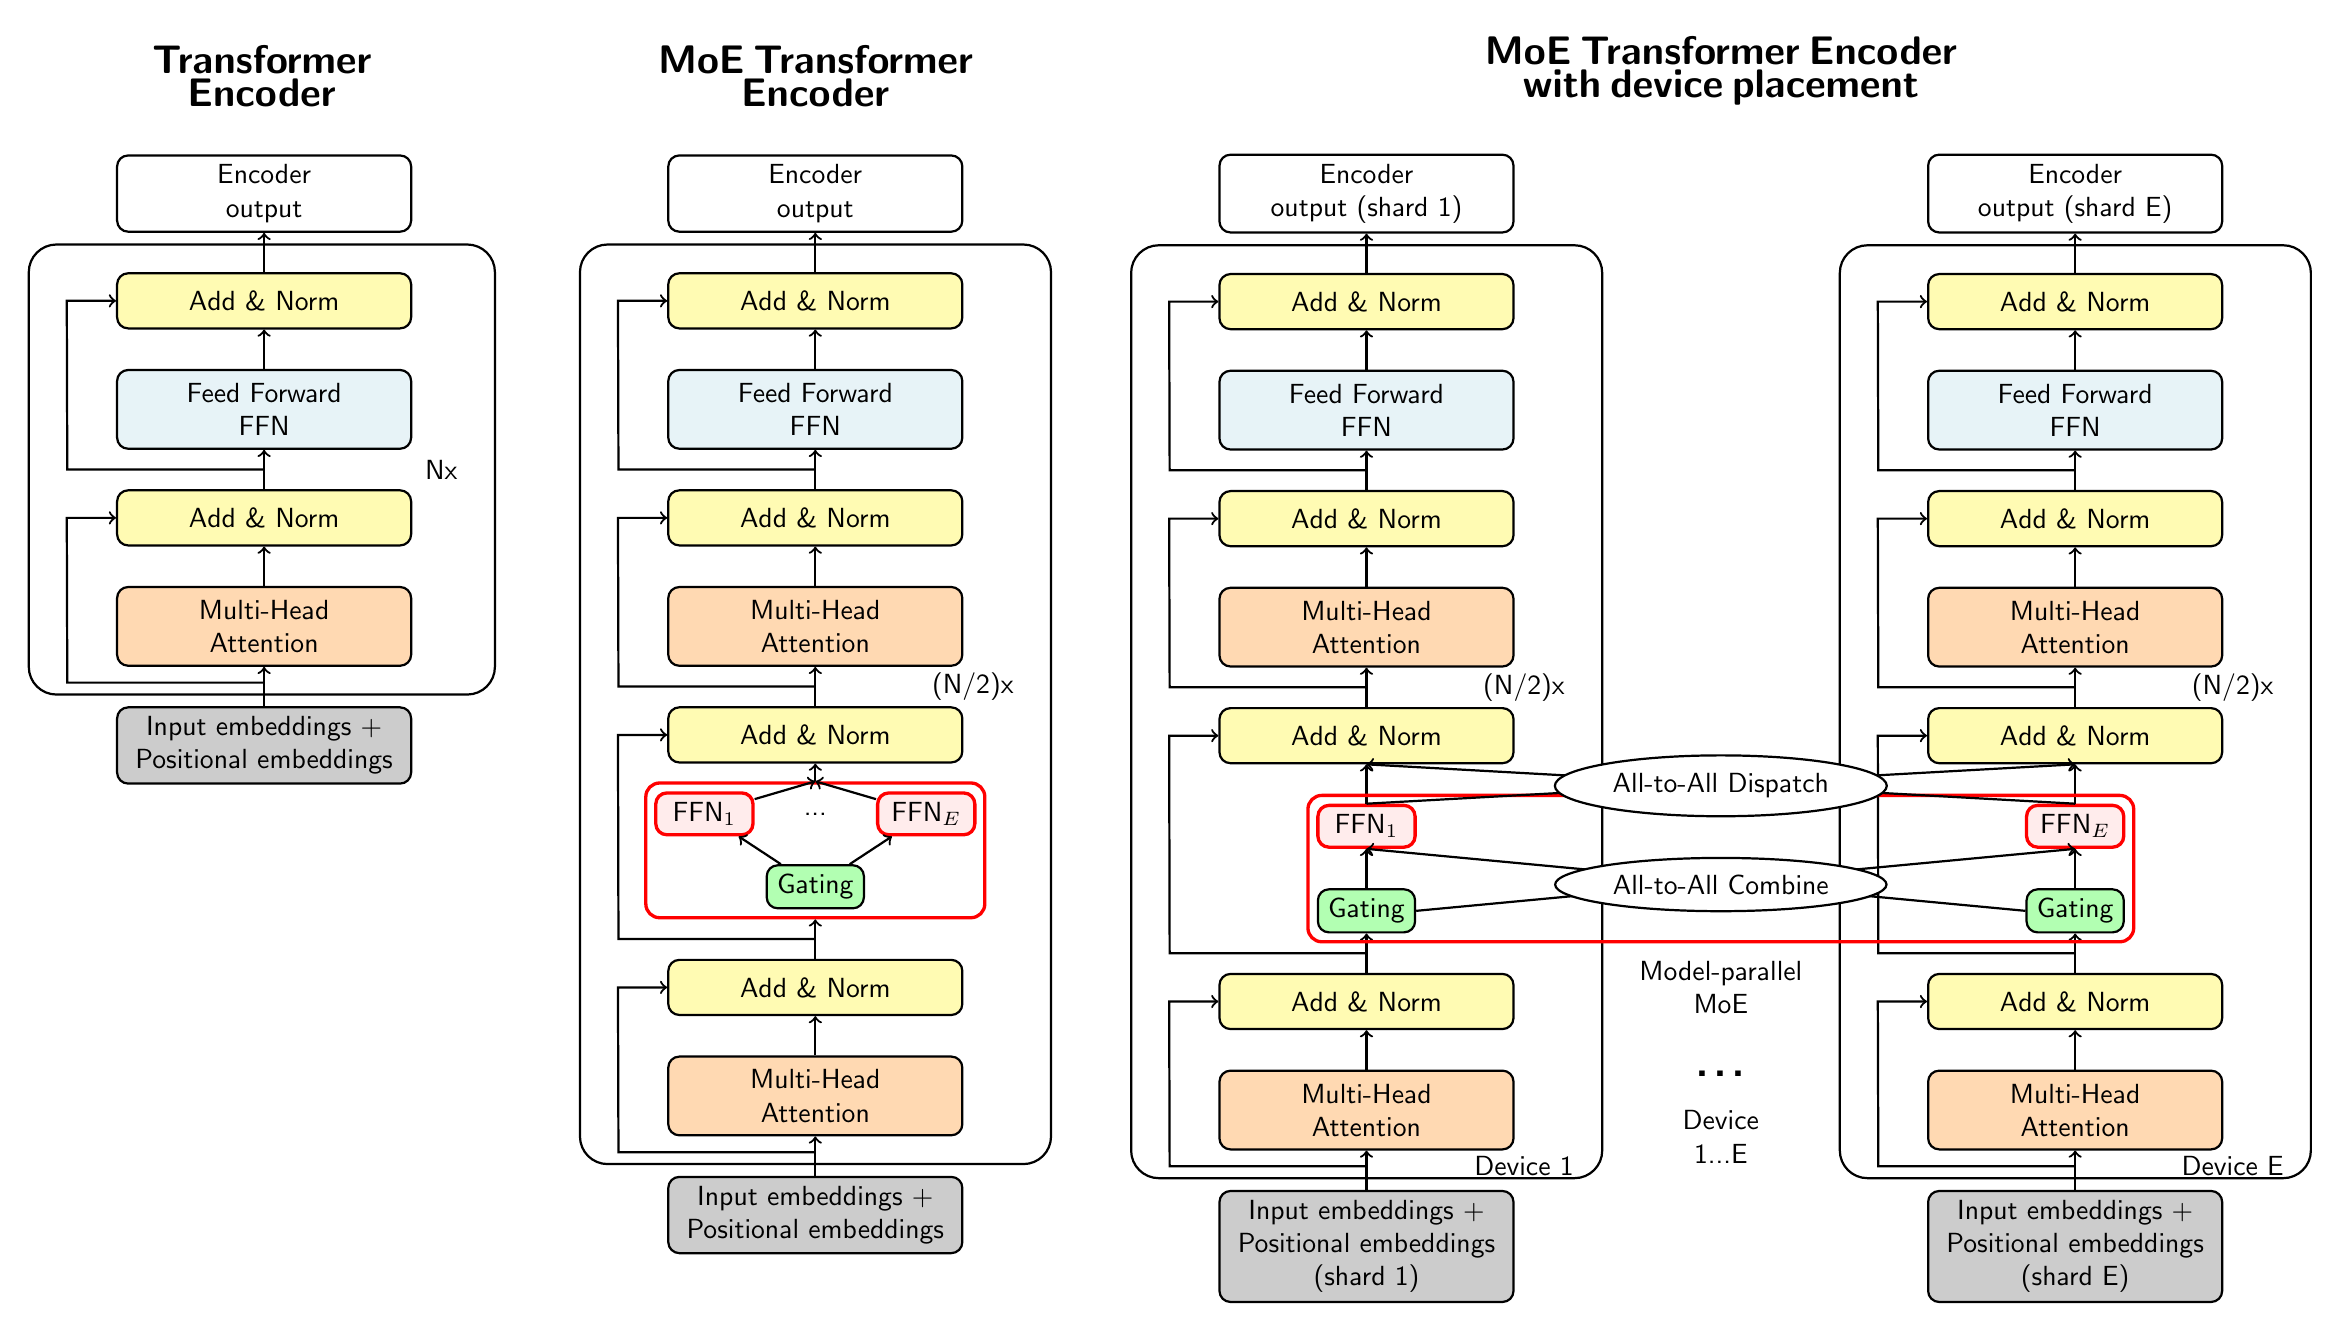
\begin{tikzpicture}[
    % 定义样式
    node distance=5mm,
    block/.style={rectangle, rounded corners, draw=black, thick, text width=3.5cm, text centered, minimum height=1cm, fill=LightBlue!30},
    addnorm/.style={rectangle, rounded corners, draw=black, thick, text width=3.5cm, text centered, minimum height=0.7cm, fill=yellow!30},
    attention/.style={rectangle, rounded corners, draw=black, thick, text width=3.5cm, text centered, minimum height=1cm, fill=orange!30},
    moe/.style={rectangle, rounded corners, draw=red, very thick, text width=1cm, text centered, minimum height=0.5cm, fill=pink!30},
    gating/.style={rectangle, rounded corners, draw=black, thick, text width=1cm, text centered, minimum height=0.5cm, fill=green!30},
    input/.style={rectangle, rounded corners, draw=black, thick, text width=3.5cm, text centered, minimum height=0.8cm, fill=gray!40},
    output/.style={rectangle, rounded corners, draw=black, thick, text width=3.5cm, text centered, minimum height=0.8cm, fill=white},
    arrow/.style={->, thick},
    dashedarrow/.style={->, thick, dashed},
    % redarrow/.style={->, red, very thick},
    container/.style={rectangle, draw=black, thick, rounded corners=10pt, inner sep=10pt},
    redcontainer/.style={rectangle, draw=red, very thick, rounded corners=5pt, inner sep=3pt},
    font=\sffamily
]

% 第一个架构 - Transformer Encoder
\begin{scope}[local bounding box=arch1]
    \node[output] (output1) {Encoder\\output};
    \node[addnorm, below=of output1] (an1_3) {Add \& Norm};
    \node[block, below=of an1_3] (ffn1) {Feed Forward\\FFN};
    \node[addnorm, below=of ffn1] (an1_2) {Add \& Norm};
    \node[attention, below=of an1_2] (mha1) {Multi-Head\\Attention};
    \node[input, below=of mha1] (input1) {Input embeddings +\\Positional embeddings};
    
    % 连接线
    \draw[arrow] (input1) -- (mha1);
    \draw[arrow] (mha1) -- (an1_2);
    \draw[arrow] (an1_2) -- (ffn1);
    \draw[arrow] (ffn1) -- (an1_3);
    \draw[arrow] (an1_3) -- (output1);
    
    % 残差连接
    \draw[arrow] ([yshift=3mm]input1.north) -- ++(-2.5,0) -- ([xshift=-6.25mm]an1_2.west) node (left_a1) {} -- (an1_2.west);
    \draw[arrow] ([yshift=2.5mm]an1_2.north) -- ++(-2.5,0) -- ([xshift=-6.25mm]an1_3.west) -- (an1_3.west);
    % Nx标记
    \node at ([yshift=2.5mm, xshift=2.25cm]an1_2.north) (Nx) {Nx};
    % 容器
    \node[container, fit=(mha1)(ffn1)(an1_2)(an1_3)(Nx)(left_a1)] (arch1_container) {};
\end{scope}

% 第二个架构 - MoE Transformer Encoder
\begin{scope}[local bounding box=arch2, xshift=7cm]
    \node[output] (output2) {Encoder\\output};
    \node[addnorm, below=of output2] (an2_4) {Add \& Norm};
    \node[block, below=of an2_4] (ffn2) {Feed Forward\\FFN};
    \node[addnorm, below=of ffn2] (an2_3) {Add \& Norm};
    \node[attention, below=of an2_3] (mha2) {Multi-Head\\Attention};
    \node[addnorm, below=of mha2] (an2_2) {Add \& Norm};
    
    % MoE部分
    \node[below=of an2_2] (ffn2_dots) {...};
    \node[moe, below=of an2_2, left=of ffn2_dots] (ffn2_1) {FFN$_1$};
    \node[moe, below=of an2_2, right=of ffn2_dots] (ffn2_E) {FFN$_E$};
    \node[gating, below=of ffn2_dots] (gating2) {Gating};
    
    % MoE容器
    \node[redcontainer, fit=(ffn2_1)(ffn2_E)(gating2)] (ffn2_moe) {};
    \node[addnorm, below=of ffn2_moe] (an2_1) {Add \& Norm};
    \node[attention, below=of an2_1] (mha2_2) {Multi-Head\\Attention};
    \node[input, below=of mha2_2] (input2) {Input embeddings +\\Positional embeddings};
    
    % 连接线
    \draw[arrow] (input2) -- (mha2_2);
    \draw[arrow] (mha2_2) -- (an2_1);
    \draw[arrow] (an2_1) -- (ffn2_moe);
    \draw[arrow] (gating2) -- (ffn2_1);
    \draw[arrow] (gating2) -- (ffn2_E);
    \draw[arrow] (ffn2_1) -- (ffn2_moe.north);
    \draw[arrow] (ffn2_E) -- (ffn2_moe.north);
    \draw[arrow] (ffn2_moe) -- (an2_2);
    \draw[arrow] (an2_2) -- (mha2);
    \draw[arrow] (mha2) -- (an2_3);
    \draw[arrow] (an2_3) -- (ffn2);
    \draw[arrow] (ffn2) -- (an2_4);
    \draw[arrow] (an2_4) -- (output2);
    
    % 残差连接
    \draw[arrow] ([yshift=3mm]input2.north) -- ++(-2.5,0) -- ([xshift=-6.25mm]an2_1.west) node (left_a2) {} -- (an2_1.west);
    \draw[arrow] ([yshift=2.5mm]an2_1.north) -- ++(-2.5,0) -- ([xshift=-6.25mm]an2_2.west) -- (an2_2.west);
    \draw[arrow] ([yshift=2.5mm]an2_2.north) -- ++(-2.5,0) -- ([xshift=-6.25mm]an2_3.west) -- (an2_3.west);
    \draw[arrow] ([yshift=2.5mm]an2_3.north) -- ++(-2.5,0) -- ([xshift=-6.25mm]an2_4.west) -- (an2_4.west);
    
    
    % (N/2)x标记
    \node at ([yshift=2.5mm, xshift=2cm]an2_2.north) (Nx2) {(N/2)x};
    
    
    % 主容器
    \node[container, fit=(mha2_2)(an2_1)(an2_2)(mha2)(an2_3)(ffn2)(an2_4)(ffn2_moe)(Nx2)(left_a2)] {};
\end{scope}

% 第三个架构 - MoE Transformer Encoder with device placement
\begin{scope}[local bounding box=arch3, xshift=14cm]
    \begin{scope}[xshift=0cm]
        \node[output] (output3_1) {Encoder\\output (shard 1)};
        \node[addnorm, below=of output3_1] (an3_4_1) {Add \& Norm};
        \node[block, below=of an3_4_1] (ffn3_1_1) {Feed Forward\\FFN};
        \node[addnorm, below=of ffn3_1_1] (an3_3_1) {Add \& Norm};
        \node[attention, below=of an3_3_1] (mha3_1_1) {Multi-Head\\Attention};
        \node[addnorm, below=of mha3_1_1] (an3_2_1) {Add \& Norm};
        
        % MoE部分
        \node[moe, below=of an3_2_1] (ffn3_1) {FFN$_1$};
        \node[gating, below=of ffn3_1] (gating3_1) {Gating};
        
        % MoE容器
        \node[addnorm, below=of gating3_1] (an3_1_1) {Add \& Norm};
        \node[attention, below=of an3_1_1] (mha3_2_1) {Multi-Head\\Attention};
        \node[input, below=of mha3_2_1] (input3_1) {Input embeddings +\\Positional embeddings\\(shard 1)};
        
        % 连接线
        \draw[arrow] (input3_1) -- (mha3_2_1);
        \draw[arrow] (mha3_2_1) -- (an3_1_1);
        \draw[arrow] (an3_1_1) -- (gating3_1);
        \draw[arrow] (gating3_1) -- (ffn3_1);
        \draw[arrow] (ffn3_1) -- (an3_2_1);
        \draw[arrow] (an3_2_1) -- (mha3_1_1);
        \draw[arrow] (mha3_1_1) -- (an3_3_1);
        \draw[arrow] (an3_3_1) -- (ffn3_1_1);
        \draw[arrow] (ffn3_1_1) -- (an3_4_1);
        \draw[arrow] (an3_4_1) -- (output3_1);
        
        % 残差连接
        \draw[arrow] ([yshift=3mm]input3_1.north) -- ++(-2.5,0) -- ([xshift=-6.25mm]an3_1_1.west) node (left_a3_1) {} -- (an3_1_1.west);
        \draw[arrow] ([yshift=2.5mm]an3_1_1.north) -- ++(-2.5,0) -- ([xshift=-6.25mm]an3_2_1.west) -- (an3_2_1.west);
        \draw[arrow] ([yshift=2.5mm]an3_2_1.north) -- ++(-2.5,0) -- ([xshift=-6.25mm]an3_3_1.west) -- (an3_3_1.west);
        \draw[arrow] ([yshift=2.5mm]an3_3_1.north) -- ++(-2.5,0) -- ([xshift=-6.25mm]an3_4_1.west) -- (an3_4_1.west);
        
        
        % (N/2)x标记
        \node at ([yshift=2.5mm, xshift=2cm]an3_2_1.north) (Nx3_1) {(N/2)x};
        % Device
        \node at ([yshift=-2mm,xshift=2cm]mha3_2_1.south) {Device 1};
        
        
        % 主容器
        \node[container, fit=(mha3_2_1)(an3_1_1)(an3_2_1)(mha3_1_1)(an3_3_1)(an3_4_1)(Nx3_1)(left_a3_1)] {};

    \end{scope}


    \begin{scope}[xshift=9cm]
        \node[output] (output3_E) {Encoder\\output (shard E)};
        \node[addnorm, below=of output3_E] (an3_4_E) {Add \& Norm};
        \node[block, below=of an3_4_E] (ffn3_1_E) {Feed Forward\\FFN};
        \node[addnorm, below=of ffn3_1_E] (an3_3_E) {Add \& Norm};
        \node[attention, below=of an3_3_E] (mha3_1_E) {Multi-Head\\Attention};
        \node[addnorm, below=of mha3_1_E] (an3_2_E) {Add \& Norm};
        
        % MoE部分
        \node[moe, below=of an3_2_E] (ffn3_E) {FFN$_E$};
        \node[gating, below=of ffn3_E] (gating3_E) {Gating};
        
        % MoE容器
        \node[addnorm, below=of gating3_E] (an3_1_E) {Add \& Norm};
        \node[attention, below=of an3_1_E] (mha3_2_E) {Multi-Head\\Attention};
        \node[input, below=of mha3_2_E] (input3_E) {Input embeddings +\\Positional embeddings\\(shard E)};
        
        % 连接线
        \draw[arrow] (input3_E) -- (mha3_2_E);
        \draw[arrow] (mha3_2_E) -- (an3_1_E);
        \draw[arrow] (an3_1_E) -- (gating3_E);
        \draw[arrow] (gating3_E) -- (ffn3_E);
        \draw[arrow] (ffn3_E) -- (an3_2_E);
        \draw[arrow] (an3_2_E) -- (mha3_1_E);
        \draw[arrow] (mha3_1_E) -- (an3_3_E);
        \draw[arrow] (an3_3_E) -- (ffn3_1_E);
        \draw[arrow] (ffn3_1_E) -- (an3_4_E);
        \draw[arrow] (an3_4_E) -- (output3_E);
        
        % 残差连接
        \draw[arrow] ([yshift=3mm]input3_E.north) -- ++(-2.5,0) -- ([xshift=-6.25mm]an3_1_E.west) node (left_a3_E) {} -- (an3_1_E.west);
        \draw[arrow] ([yshift=2.5mm]an3_1_E.north) -- ++(-2.5,0) -- ([xshift=-6.25mm]an3_2_E.west) -- (an3_2_E.west);
        \draw[arrow] ([yshift=2.5mm]an3_2_E.north) -- ++(-2.5,0) -- ([xshift=-6.25mm]an3_3_E.west) -- (an3_3_E.west);
        \draw[arrow] ([yshift=2.5mm]an3_3_E.north) -- ++(-2.5,0) -- ([xshift=-6.25mm]an3_4_E.west) -- (an3_4_E.west);
        
        
        % (N/2)x标记
        \node at ([yshift=2.5mm, xshift=2cm]an3_2_E.north) (Nx3_E) {(N/2)x};
        % Device
        \node at ([yshift=-2mm,xshift=2cm]mha3_2_E.south) {Device E};
        
        % 主容器
        \node[container, fit=(mha3_2_E)(an3_1_E)(an3_2_E)(mha3_1_E)(an3_3_E)(an3_4_E)(Nx3_E)(left_a3_E)] {};
    \end{scope}
        
    % MoE容器
    \node[redcontainer, fit=(ffn3_1)(ffn3_E)(gating3_1)(gating3_E)] (ffn3) {};
    \node[below=1mm of ffn3, align=center] {Model-parallel\\MoE};

    % 设备标记
    \node[below=1.5cm of ffn3] {\Huge...};
    \node[below=2cm of ffn3, align=center] {Device\\1...E};

    % All-to-All连接
    \draw[arrow] (gating3_1.east) -- (ffn3_E.south);
    \draw[arrow] (gating3_E.west) -- (ffn3_1.south);
    \draw[arrow] (ffn3_1.north) -- (an3_2_E.south);
    \draw[arrow] (ffn3_E.north) -- (an3_2_1.south);

    \node[ellipse,thick,draw,fill=white, above=-3mm of ffn3] {All-to-All Dispatch};
    \node[ellipse,thick,draw,fill=white, below=-1.1cm of ffn3] {All-to-All Combine};
\end{scope}

% 架构标题
\node[text width=5cm, above=0.5cm of arch1.north, align=center] {\Large \textbf{Transformer\\Encoder}};
\node[text width=5cm, above=0.5cm of arch2.north, align=center] {\Large \textbf{MoE Transformer\\Encoder}};
\node[text width=8cm, above=0.5cm of arch3.north, align=center] {\Large \textbf{MoE Transformer Encoder\\with device placement}};

% 箭头连接三个架构

% TODO

\end{tikzpicture}
\end{document}